
\begin{question}
Please make a frequency table and a frequency histogram from the
following (unsorted) continuous data by rounding to the nearest integer.

\begin{longtable}[]{@{}rrrrr@{}}
\toprule
\endhead
37.4419 & 36.6627 & 38.5894 & 36.6057 & 37.8983\tabularnewline
33.2985 & 33.5310 & 34.5369 & 38.4055 & 34.2746\tabularnewline
34.2033 & 34.9203 & 35.2866 & 36.6045 & 37.7256\tabularnewline
34.7470 & 36.4322 & 35.8255 & 32.7223 & 34.5098\tabularnewline
\bottomrule
\end{longtable}
\end{question}

\begin{solution}
Make a frequency table.

\begin{longtable}[]{@{}rr@{}}
\toprule
bin & frequency\tabularnewline
\midrule
\endhead
33 & 2\tabularnewline
34 & 3\tabularnewline
35 & 5\tabularnewline
36 & 2\tabularnewline
37 & 4\tabularnewline
38 & 3\tabularnewline
39 & 1\tabularnewline
\bottomrule
\end{longtable}

Make the histogram.

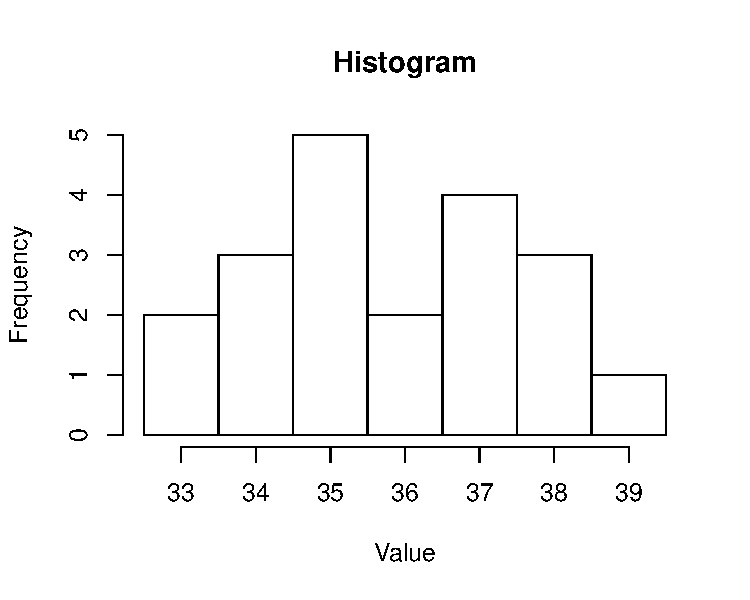
\includegraphics{barchart-1.pdf}\\
\end{solution}

